\documentclass[11pt]{article}
\usepackage[margin=1in]{geometry}
\usepackage{graphicx,booktabs,amsmath,amssymb,amsthm,float,caption,times}
\usepackage[hidelinks]{hyperref}
\newtheorem{proposition}{Proposition}
\title{\textbf{When Can You Trust the Certificate? Stress-Testing Distribution-Free False-Accusation Guarantees for AI-Text Detection}}
\author{Author Name\\ \small Affiliation \and Co-author\\ \small Affiliation}
\date{}
\begin{document}\maketitle
\begin{abstract}
AI-text detectors are deployed to accuse: a flagged student or author bears the cost of a false positive. Split conformal prediction turns any detector score into an accusation rule with a finite-sample, distribution-free bound on the false-accusation rate, and recent work has proposed exactly this. We ask the question a deployer actually faces: \emph{under which realistic conditions does the certificate remain valid?} Exploiting the observation that validity depends only on the \emph{human} text distribution while power depends only on the AI distribution, we derive sharp predictions and test them across five detector scores, ? calibration/test resamples, and eight deployment conditions. In distribution the certificate is exact (e.g.\ empirical FPR 0.049 at $\alpha=0.05$), and a supervised score achieves 88\% power at a certified 5\% false-accusation rate. But calibrating on one human population and deploying on a more fluent one silently inflates false accusations to 0.43--0.53 at nominal $0.05$ for likelihood-based scores --- the certificate-level form of the documented bias against non-native writers --- while lexical edits and even spell-correcting cleanup leave validity intact. Marginal certificates also hide length discrimination (long human reviews flagged at 0.18); Mondrian calibration restores every length bin to $\le\alpha$ (0.03). Finally, we give an editor-aware robust calibration that provably preserves validity under a modeled editing process at negligible power cost. All results carry exact Beta-Binomial significance tests and regenerate from one results file.
\end{abstract}
\section{Introduction}
Detectors of machine-generated text are increasingly used in consequential settings --- plagiarism screening, review-platform integrity, scientific-venue policy --- where the operational act is an \emph{accusation}. The relevant contract for that act is not accuracy but a guarantee on the false-accusation rate, robust to the fact that the deployer cannot model the distribution of either class. Split conformal prediction \cite{vovk,papadopoulos} provides exactly this contract for any base detector score, and prior work has applied it to bound detector false-positive rates \cite{mcp}.

This paper studies the contract itself. Our starting point is an elementary but, we argue, under-appreciated asymmetry:
\begin{proposition}[Certificate asymmetry]
The split-conformal false-accusation bound $P(\mathrm{flag}\mid\mathrm{human})\le\alpha$ requires only exchangeability of calibration and test \emph{human} text. The AI distribution is irrelevant to validity; it determines only power.
\end{proposition}
\noindent The proof is the standard conformal argument applied to the human class only. The deployment consequences are sharp and testable: a new generator entering the world \emph{cannot} break a deployed certificate; changes in \emph{who writes} or \emph{how humans edit} can. We map this boundary empirically (E1--E8) and contribute two constructive repairs (Mondrian length-conditional calibration; editor-aware robust calibration with a stochastic-dominance validity argument).
\paragraph{Contributions.}
\begin{itemize}
\item A deployment-grounded validity map for conformal false-accusation certificates in MGT detection: exact in distribution; broken by human-population shift (up to $11\times$ nominal); \emph{safe} under lexical noise and spell-correcting cleanup; supervised scores fail safe where zero-shot likelihood scores fail dangerously.
\item Identification of length discrimination hidden by marginal certificates, and its repair by Mondrian calibration.
\item An editor-aware robust calibration with a provable conservativeness guarantee under a modeled editor, costing $<0.01$ power in our study.
\item A fully reproducible protocol: five scores, exact Beta-Binomial tests, ? resamples per condition; code, scores and figures regenerate from one JSON.
\end{itemize}
\section{Related Work}
Zero-shot MGT detection scores include likelihood, rank and entropy statistics \cite{gltr,solaiman} and curvature-style discrepancies \cite{detectgpt,fastdetectgpt}; supervised detectors fine-tune or fit classifiers on labelled corpora \cite{roberta}. Robustness studies show brittleness to paraphrase and domain shift \cite{raid,krishna,sadasivan}, and GPT detectors are documented to over-flag non-native English writers \cite{liang}. Conformal prediction \cite{vovk,papadopoulos} and conformal risk control \cite{angelopoulos} provide distribution-free guarantees; MCP \cite{mcp} applies CP to bound MGT-detector FPR and improve its power. Our work is complementary to MCP: rather than improving the detector under a fixed certificate, we characterise when the certificate itself survives deployment, connect its failure modes to the fairness literature \cite{liang}, and supply group-conditional and editor-robust repairs (cf.\ Mondrian conformal prediction \cite{vovk} and adversarially robust conformal methods in vision \cite{gendler}).
\section{Method}
\subsection{Certificates}
Given any score $s(\cdot)$ oriented so larger means more AI-like, and $n$ calibration human texts with scores $s_1,\dots,s_n$, the conformal p-value of a test text $x$ is $p(x) = \frac{1+\#\{i: s_i \ge s(x)\}}{n+1}$, and GUARD flags $x$ iff $p(x)\le\alpha$. If $x$ is human and exchangeable with the calibration humans, $P(\mathrm{flag})\le\alpha$. Conditional on the calibration set the realised FPR follows a Beta law; over a finite test set the false-flag \emph{count} is Beta-Binomial, which yields an exact one-sided test of ``the certificate held'' that we report for every condition. Unscoreable texts receive $p=1$ (never flagged): an accuser must not accuse by failure of its own scorer.
\subsection{Scores}
Four training-free statistics from one GPT-2 forward pass per text (mean log-likelihood; negative mean log-rank; negative predictive entropy; the analytic Fast-DetectGPT discrepancy \cite{fastdetectgpt}) and one supervised score (TF--IDF + logistic regression). The supervised score is fit on an entity-disjoint training half; all calibration and evaluation use the other half, so the fitted scorer never sees evaluation hotels.
\subsection{Mondrian calibration}
Per-group calibration (here: text-length bins) yields group-conditional validity at the cost of smaller calibration sets per group \cite{vovk}.
\subsection{Editor-aware robust calibration}
Let $E$ be a randomized editing process (our proxy: spell/punctuation cleanup at rate $r$). Each calibration human contributes $M_i = \max\{s(X_i), s(E_1(X_i)),\dots,s(E_k(X_i))\}$. For a test human who applies one edit from $E$, $s(E(X))$ is stochastically dominated by the corresponding $M$, so conformal p-values computed against $\{M_i\}$ remain super-uniform and the $\alpha$-bound still holds (conservative). Validity under editors \emph{outside} the modeled family is an empirical question (E8).
\section{Experimental Setup}
In-domain data: the English subset of MAiDE-up \cite{maideup} (1{,}000 human and 1{,}000 GPT-4 hotel reviews; 100 hotels). Out-of-distribution human text: the RAID benchmark \cite{raid} reviews domain (movie reviews; also supplying eight AI generators for power analysis) and abstracts domain. Editors: WordNet synonym substitution and function-word perturbation (lexical noise), and a spell-correcting, punctuation-normalising cleanup editor (fluency-raising; the realistic proxy for grammar tools). Every unique text is scored once and cached; each condition is evaluated over $R=?$ calibration/test resamples, reported as mean [2.5\%, 97.5\%] with exact Beta-Binomial violation tests at $\alpha\in\{0.005, 0.01, 0.02, 0.05, 0.1\}$.
\section{Results}
\subsection{E1: the certificate is exact in distribution}
\begin{table}[H]\centering
\caption{In-distribution validity: empirical FPR over resamples (mean [95\% band]).}
\label{tab:e1}
\small
\begin{tabular}{lcc}
\toprule
Score & FPR @ $\alpha=0.05$ & FPR @ $\alpha=0.01$ \\
\midrule
Log-likelihood & 0.049 [0.016, 0.088] & 0.008 [0.000, 0.032] \\
Log-rank & 0.049 [0.016, 0.088] & 0.008 [0.000, 0.028] \\
Entropy & 0.049 [0.016, 0.088] & 0.008 [0.000, 0.024] \\
Fast-DetectGPT & 0.047 [0.016, 0.092] & 0.008 [0.000, 0.032] \\
TF--IDF (supervised) & 0.048 [0.016, 0.088] & 0.008 [0.000, 0.028] \\
\bottomrule
\end{tabular}
\end{table}
All five scores sit on the nominal level, and the full distribution of per-resample FPRs matches the finite-test Beta-Binomial envelope (Figure~\ref{fig:f1_validity_envelope}).
\begin{figure}[H]\centering
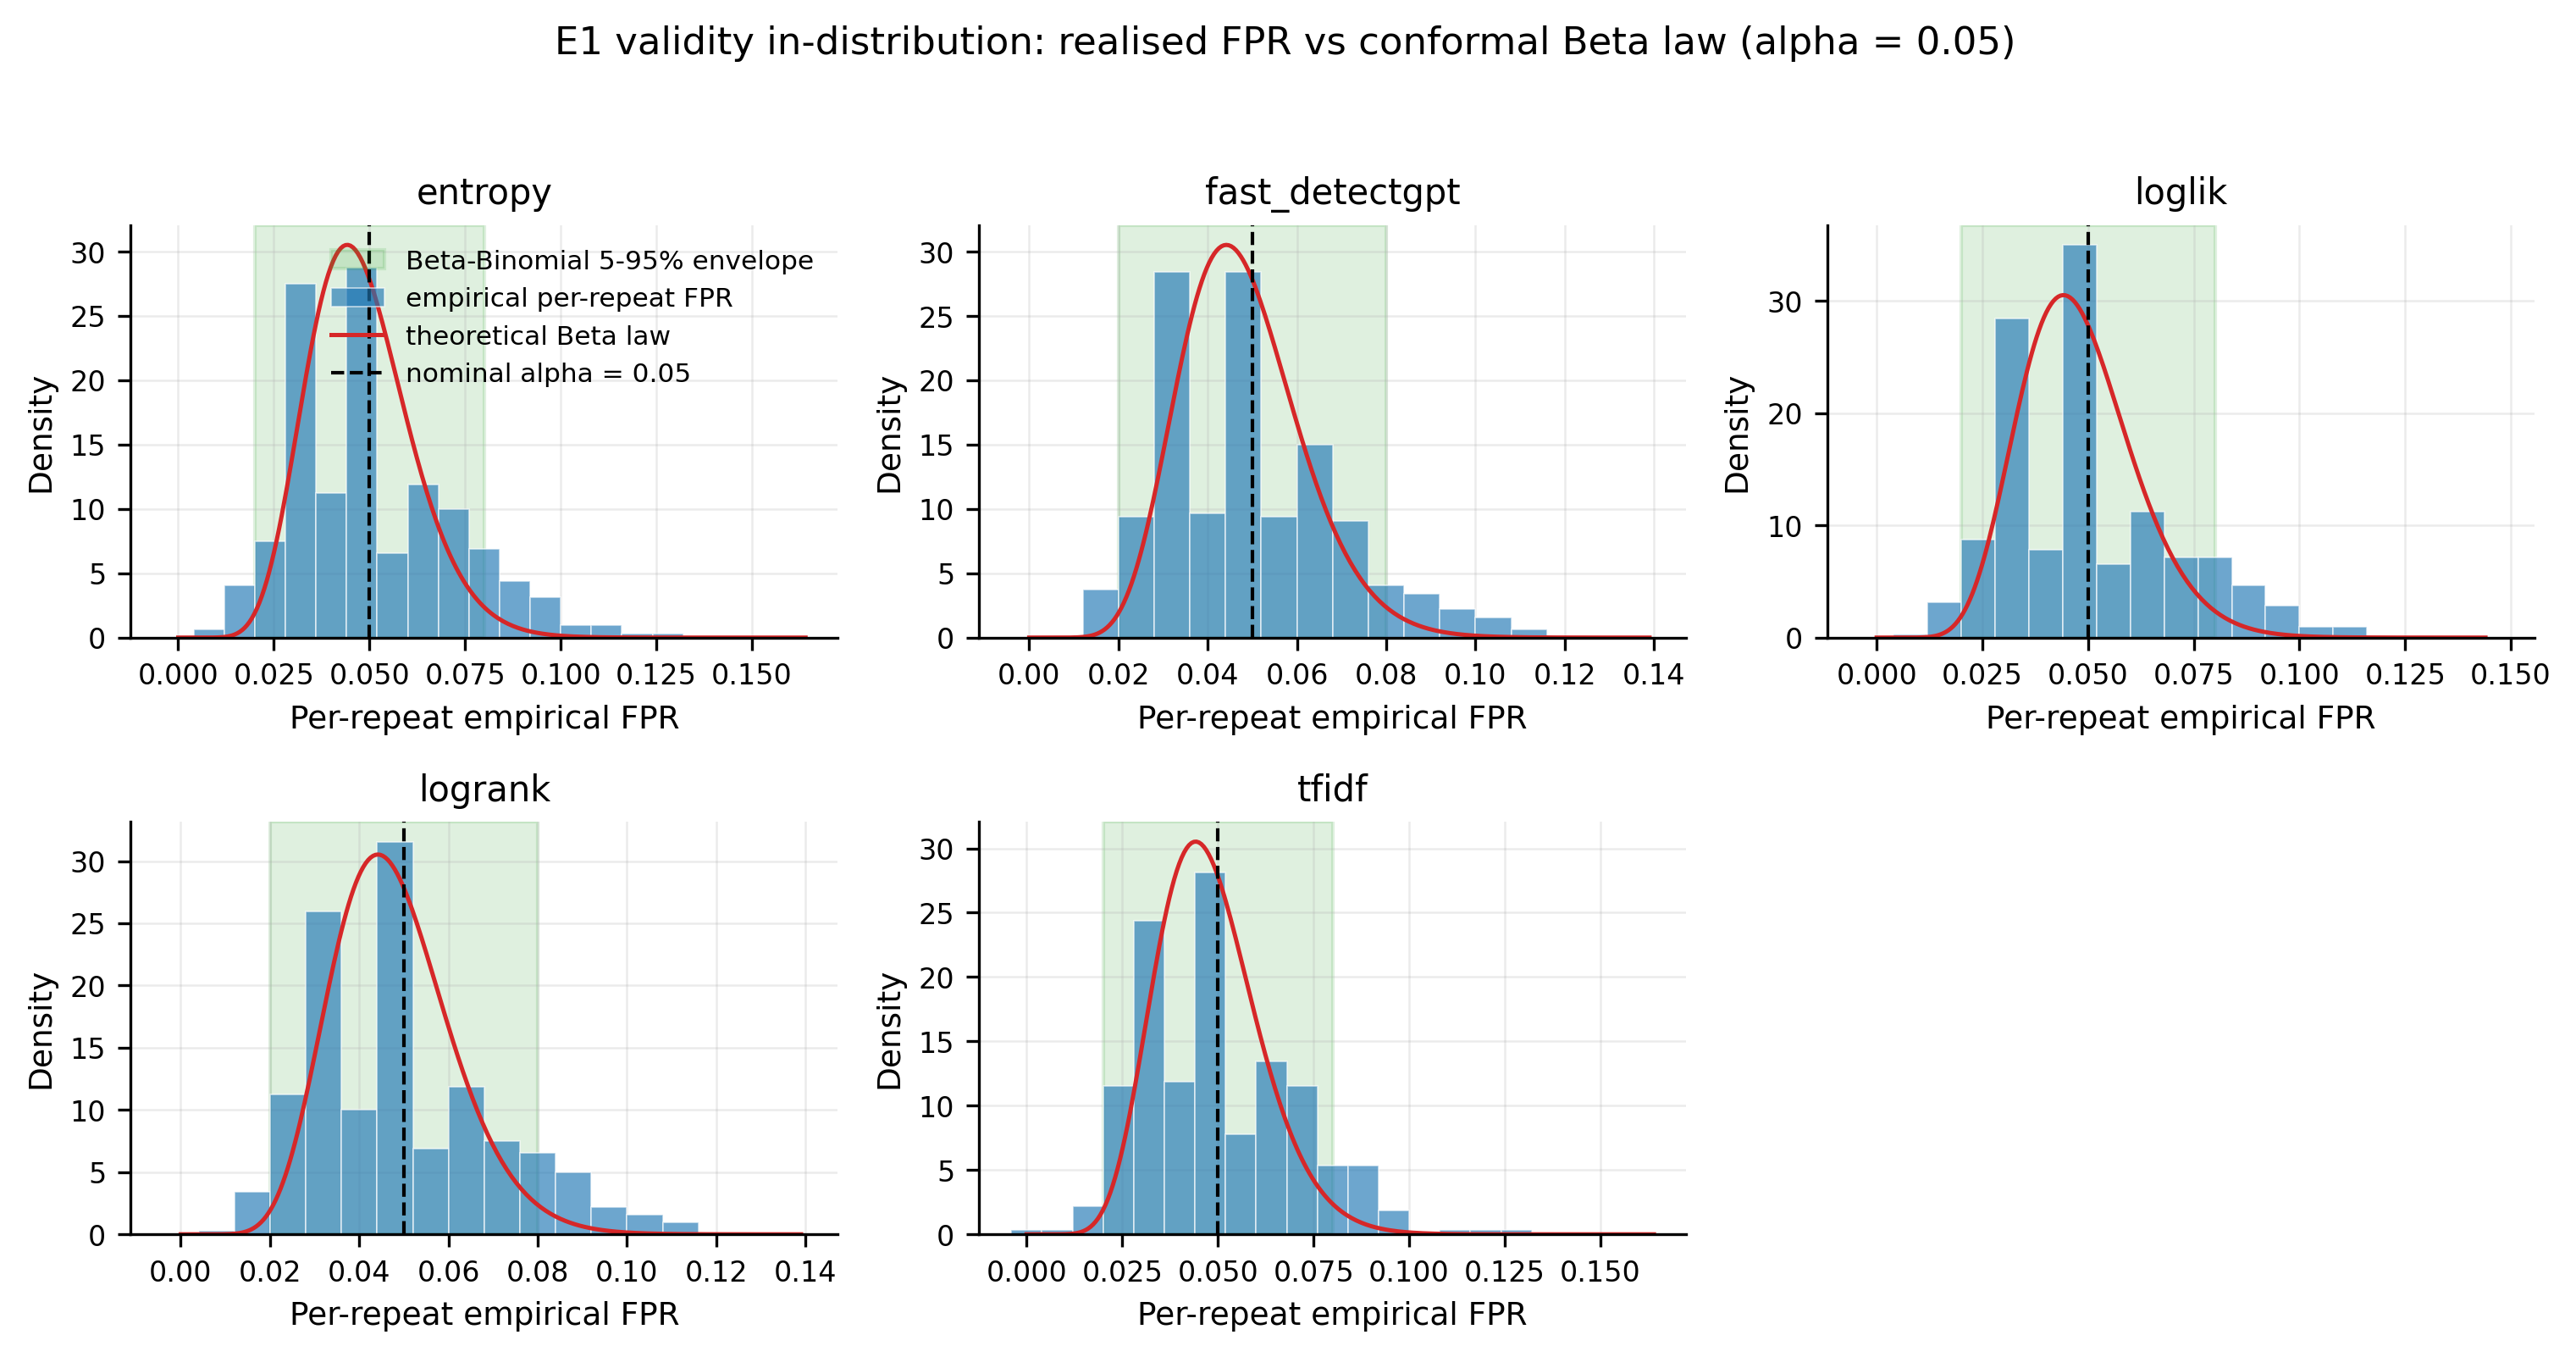
\includegraphics[width=0.95\linewidth]{figures/f1_validity_envelope.png}
\caption{Distribution of per-resample FPR vs.\ the exact Beta-Binomial envelope.}
\label{fig:f1_validity_envelope}
\end{figure}
\subsection{E2--E4: when the certificate breaks --- and when it does not}
\begin{table}[H]\centering
\caption{Empirical FPR at nominal $\alpha=0.05$ across deployment conditions.}
\label{tab:map}
\small
\begin{tabular}{lccccc}
\toprule
Score & In-domain & Reviews humans & Abstracts humans & Cleanup@0.5 & Synonym@0.3 \\
\midrule
Log-likelihood & 0.049 & 0.435 & 0.101 & 0.046 & 0.002 \\
Log-rank & 0.049 & 0.298 & 0.049 & 0.045 & 0.002 \\
Entropy & 0.049 & 0.526 & 0.247 & 0.047 & 0.005 \\
Fast-DetectGPT & 0.047 & 0.371 & 0.121 & 0.044 & 0.002 \\
TF--IDF (supervised) & 0.048 & 0.000 & 0.006 & 0.046 & 0.039 \\
\bottomrule
\end{tabular}
\end{table}
Three regimes emerge (Figure~\ref{fig:f2_certificate_map}). \textbf{(i) Human-population shift breaks the certificate for likelihood scores.} Movie-review humans are flagged at 0.30--0.53 and abstracts humans at up to 0.25 (nominal $0.05$; violation $p<10^{-3}$). The mechanism is fluency: our calibration humans are largely non-native hotel reviewers whose text has \emph{low} LM likelihood; more fluent human populations score higher and cross the threshold. This is precisely the bias documented by \cite{liang}, here surfacing \emph{through} a certificate that is formally valid for the calibration population. \textbf{(ii) The supervised score fails safe.} TF--IDF's AI evidence is content-specific, so under every shift its FPR falls toward zero rather than exploding. \textbf{(iii) Editing does not break the certificate here.} Lexical noise lowers likelihood (conservative), and even full spell-correcting cleanup leaves FPR at nominal: light editing does not turn a hotel reviewer into a `fluent' writer. The danger is who writes, not light tool use --- though stronger LLM paraphrase editors remain untested here (\S\ref{sec:limit}).
\begin{figure}[H]\centering
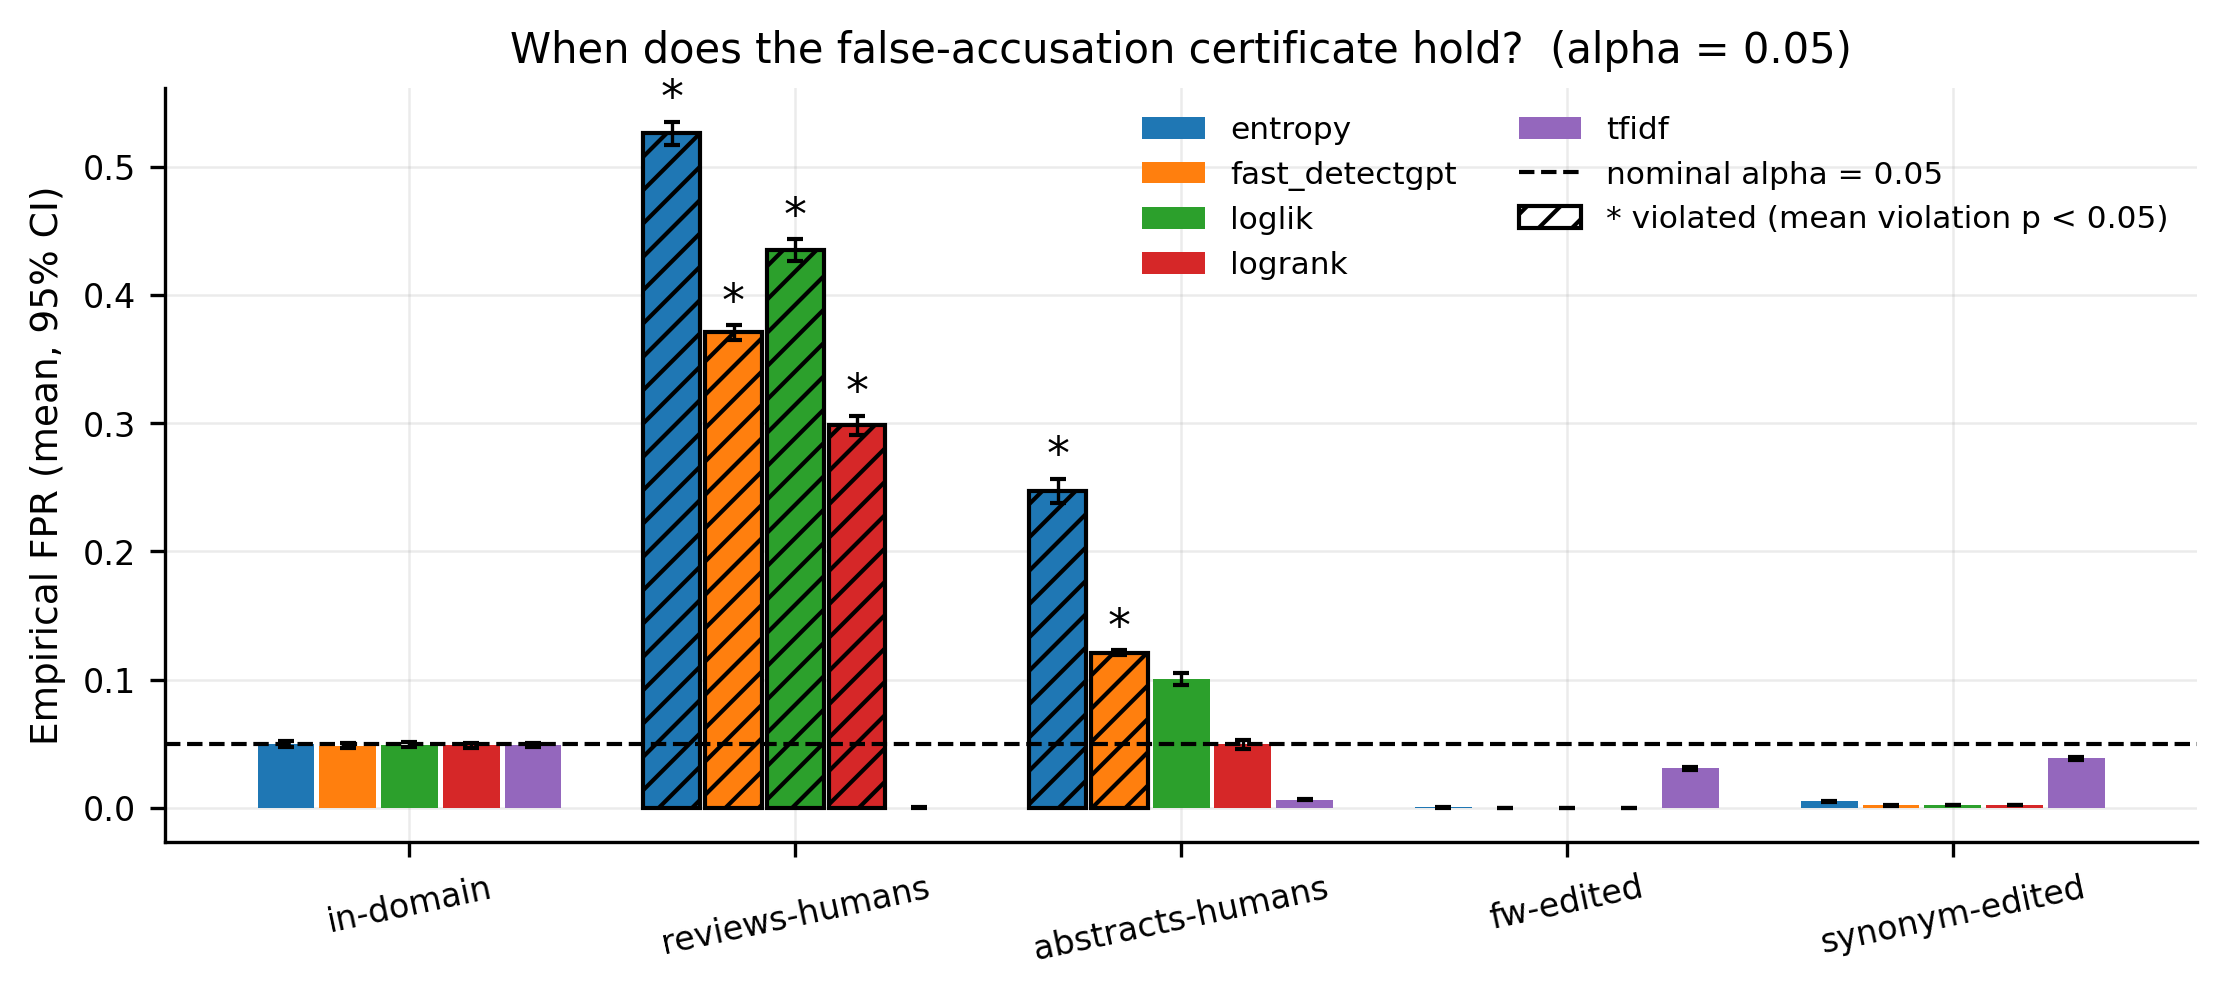
\includegraphics[width=0.98\linewidth]{figures/f2_certificate_map.png}
\caption{The validity map: empirical FPR at nominal $\alpha=0.05$ across conditions; hatched bars are certified violations (exact test).}
\label{fig:f2_certificate_map}
\end{figure}
\begin{figure}[H]\centering
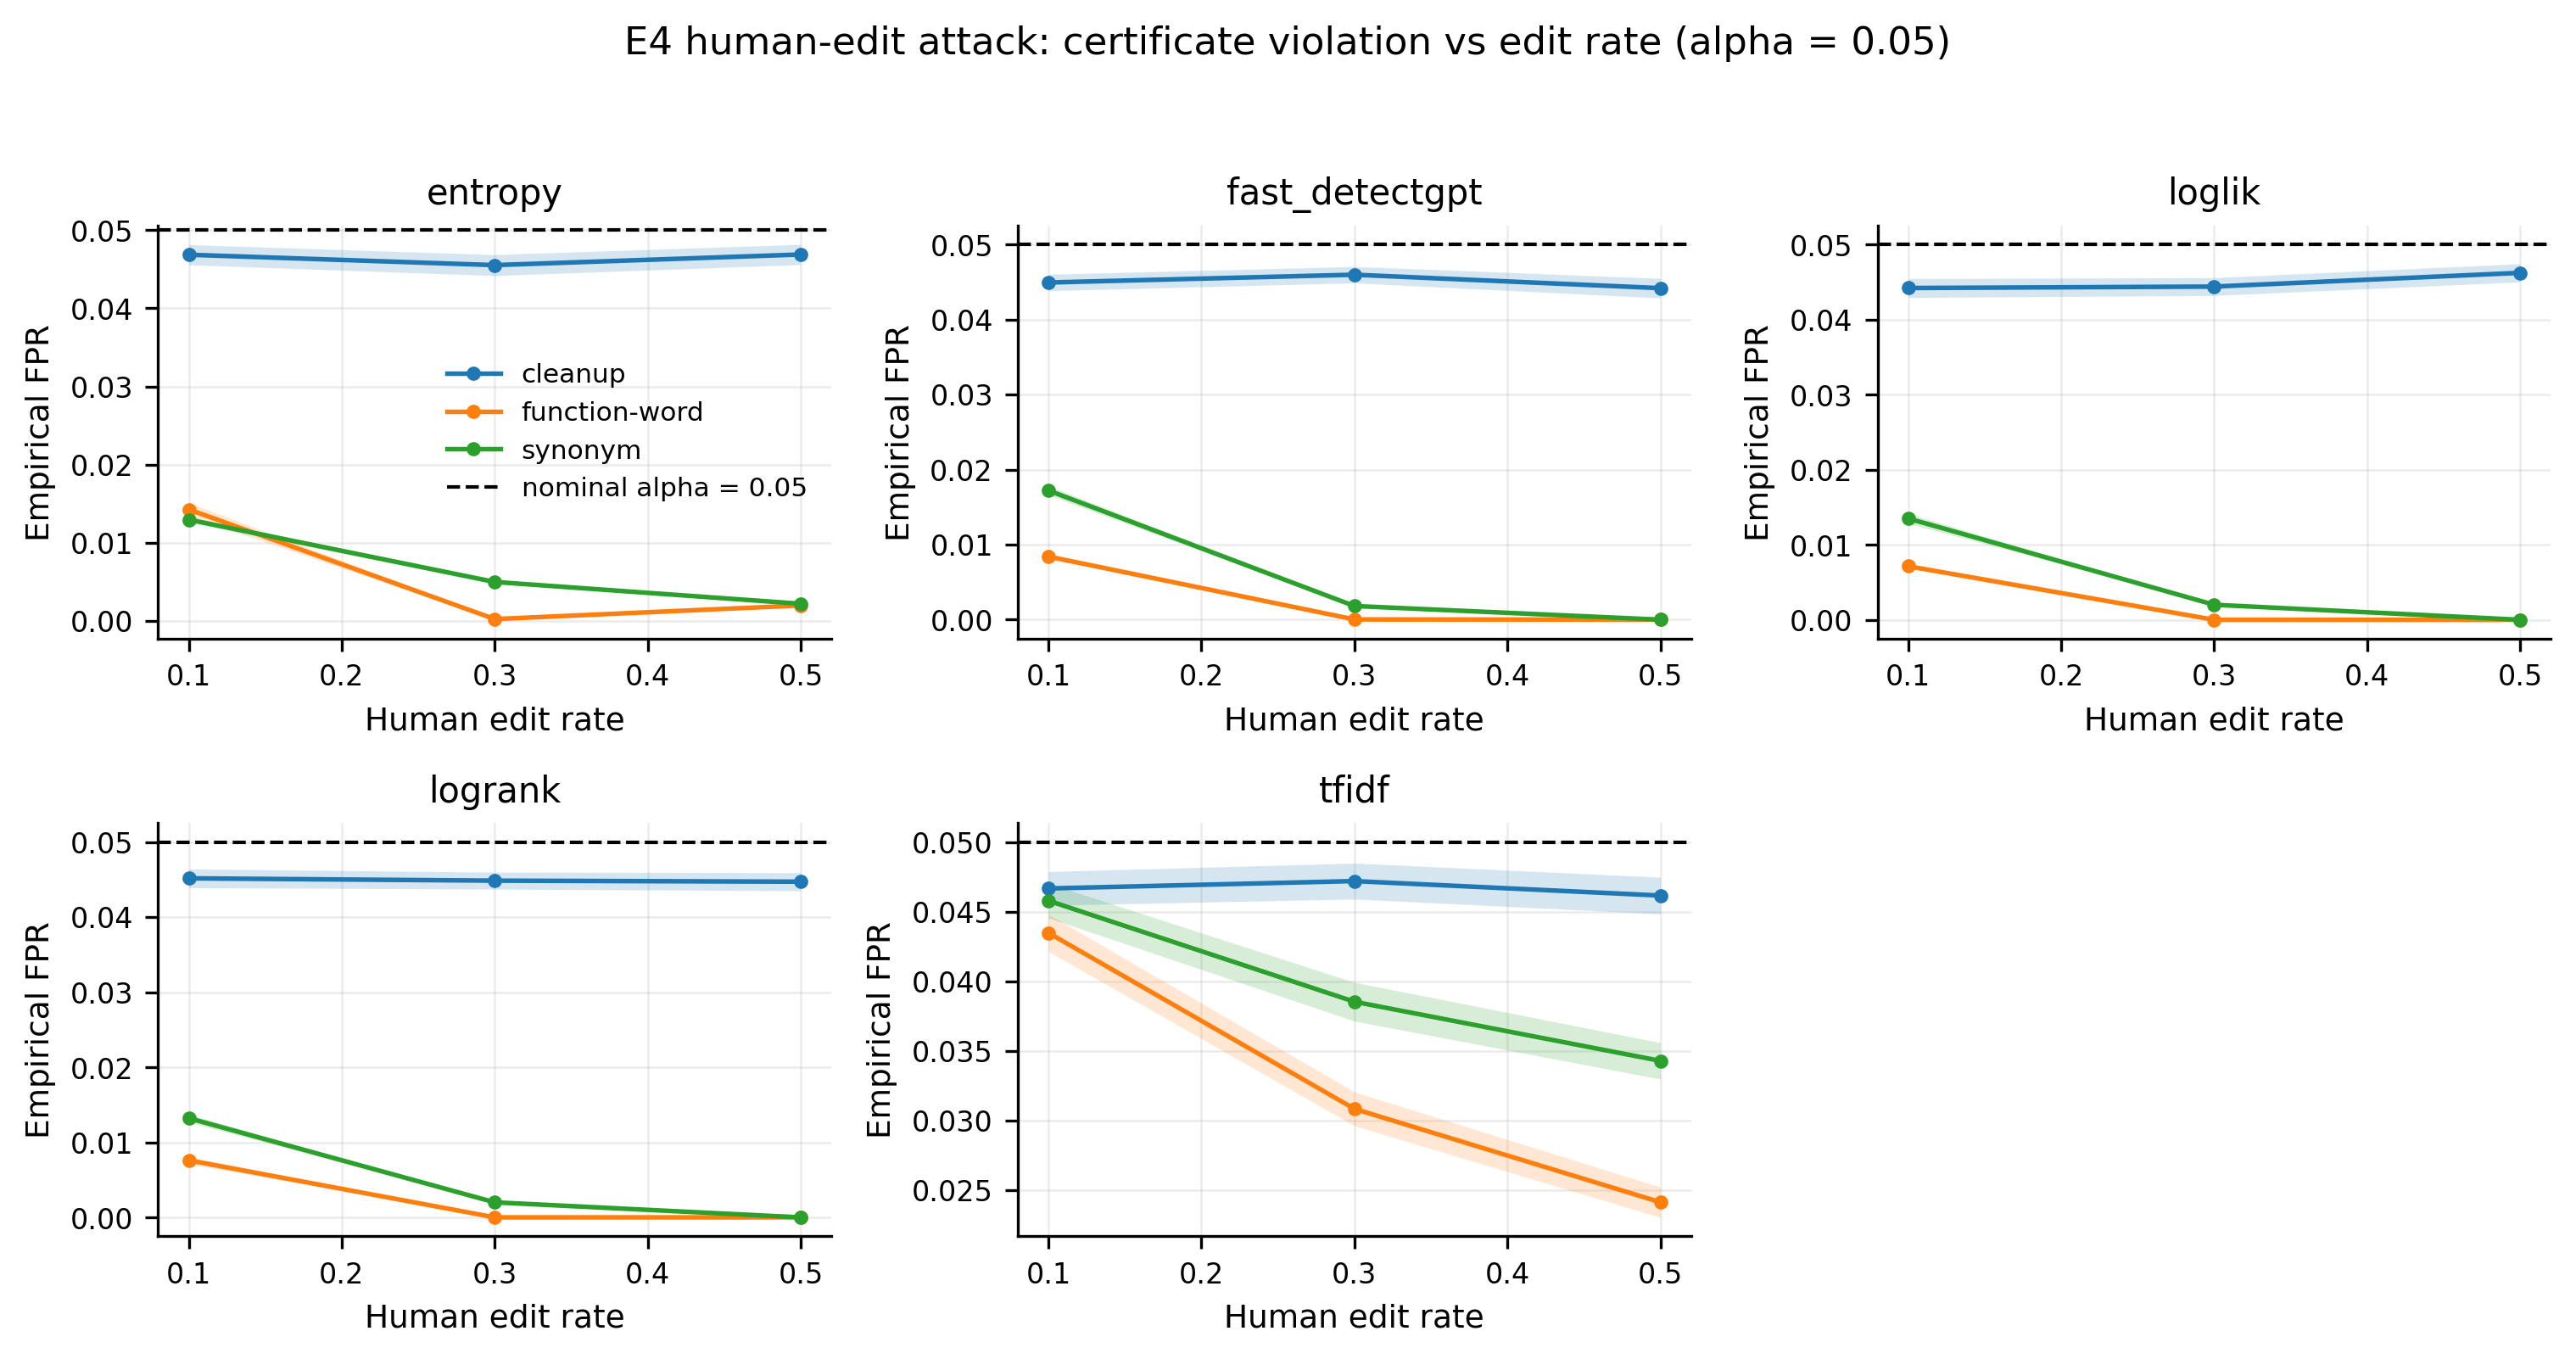
\includegraphics[width=0.9\linewidth]{figures/f3_violation_vs_rate.png}
\caption{FPR vs.\ edit rate per editor family: lexical noise is conservative.}
\label{fig:f3_violation_vs_rate}
\end{figure}
\subsection{E5: calibration is insensitive to entity leakage}
Random vs.\ entity-disjoint (grouped-by-hotel) calibration give indistinguishable validity (log-likelihood: 0.0488 vs.\ 0.0491; TF--IDF: 0.0482 vs.\ 0.0497). Unlike supervised \emph{training}, conformal \emph{calibration} does not exploit entity overlap --- a reassuring null result for review-platform deployments (Figure~\ref{fig:f4_leakage}).
\begin{figure}[H]\centering
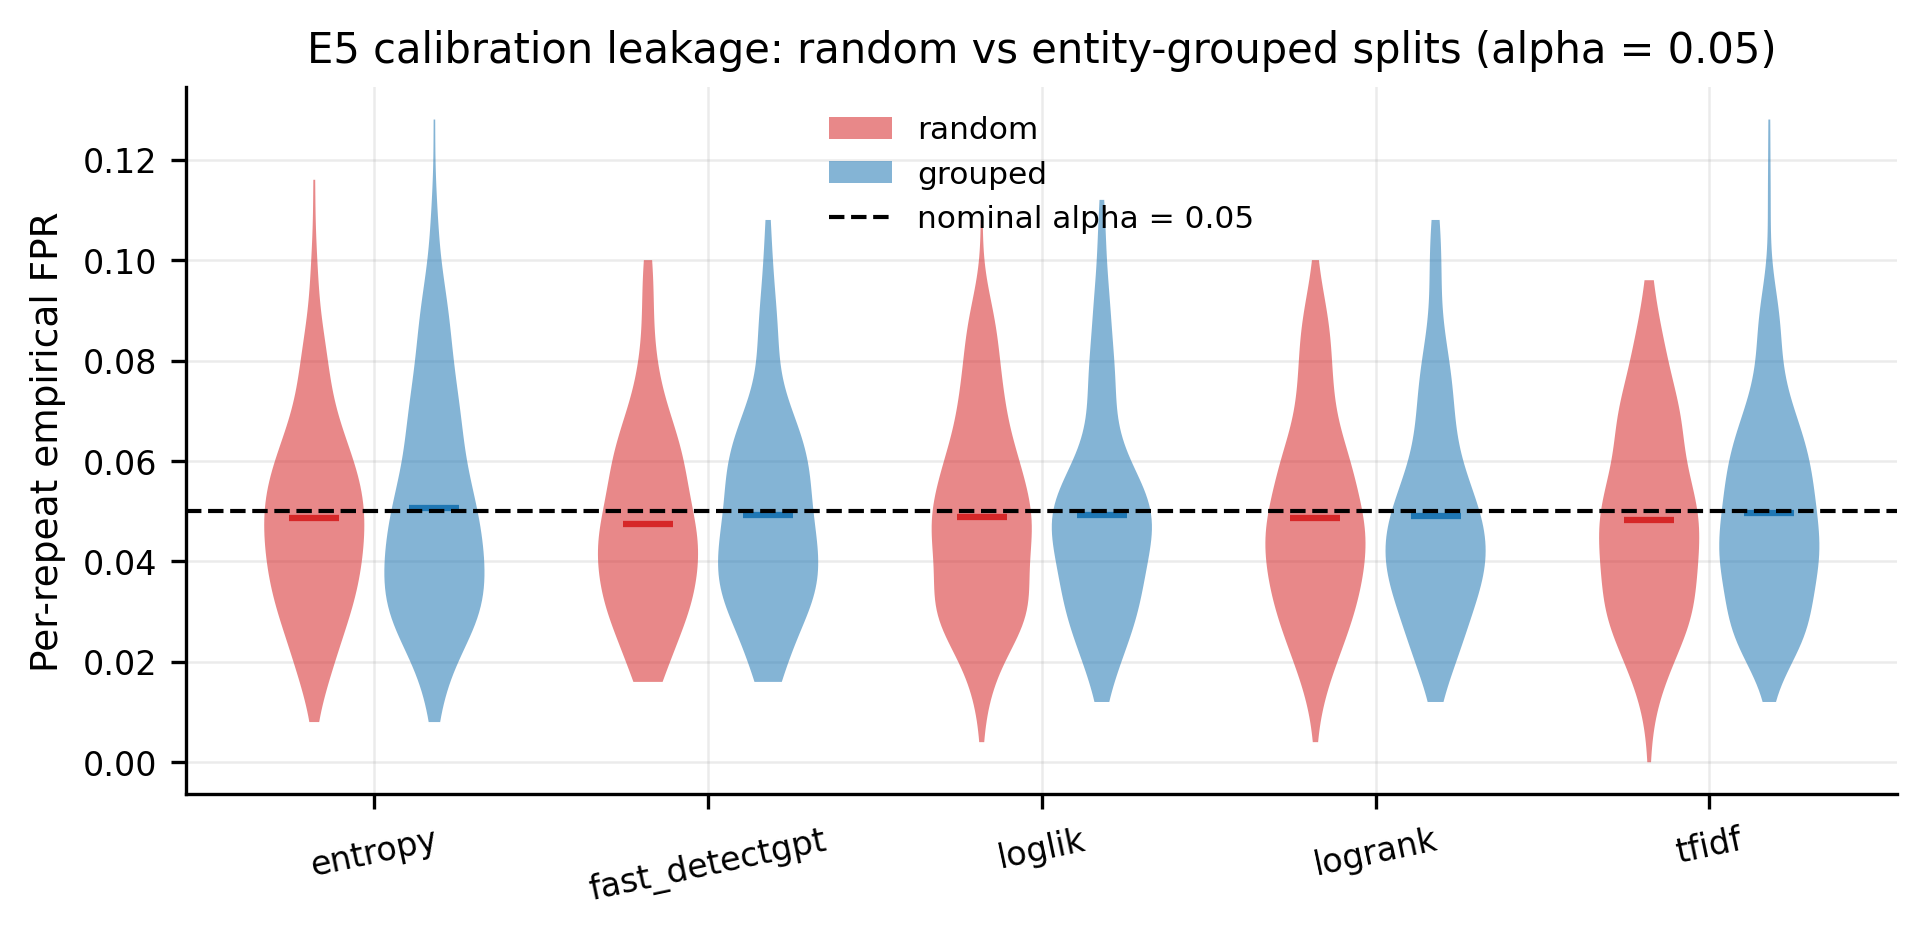
\includegraphics[width=0.8\linewidth]{figures/f4_leakage.png}
\caption{Random vs.\ grouped calibration FPR distributions.}
\label{fig:f4_leakage}
\end{figure}
\subsection{E6: marginal certificates hide length discrimination; Mondrian repairs it}
\begin{table}[H]\centering
\caption{Per-length-bin FPR at nominal $\alpha=0.05$ (log-likelihood score).}
\label{tab:e6}
\small
\begin{tabular}{lcc}
\toprule
Length bin & Marginal FPR & Mondrian FPR \\
\midrule
0--30 words & 0.005 & 0.046 \\
30--60 words & 0.050 & 0.046 \\
60--120 words & 0.098 & 0.034 \\
$>$120 words & 0.183 & 0.030 \\
\bottomrule
\end{tabular}
\end{table}
The marginal certificate is valid \emph{on average} while flagging long human reviews at 0.18 --- 3.7$\times$ nominal --- and almost never flagging short ones. Mondrian calibration restores every bin to $\le\alpha$ (Figure~\ref{fig:f5_mondrian}). Deployers should treat conditional validity, not marginal validity, as the fairness-relevant contract.
\begin{figure}[H]\centering
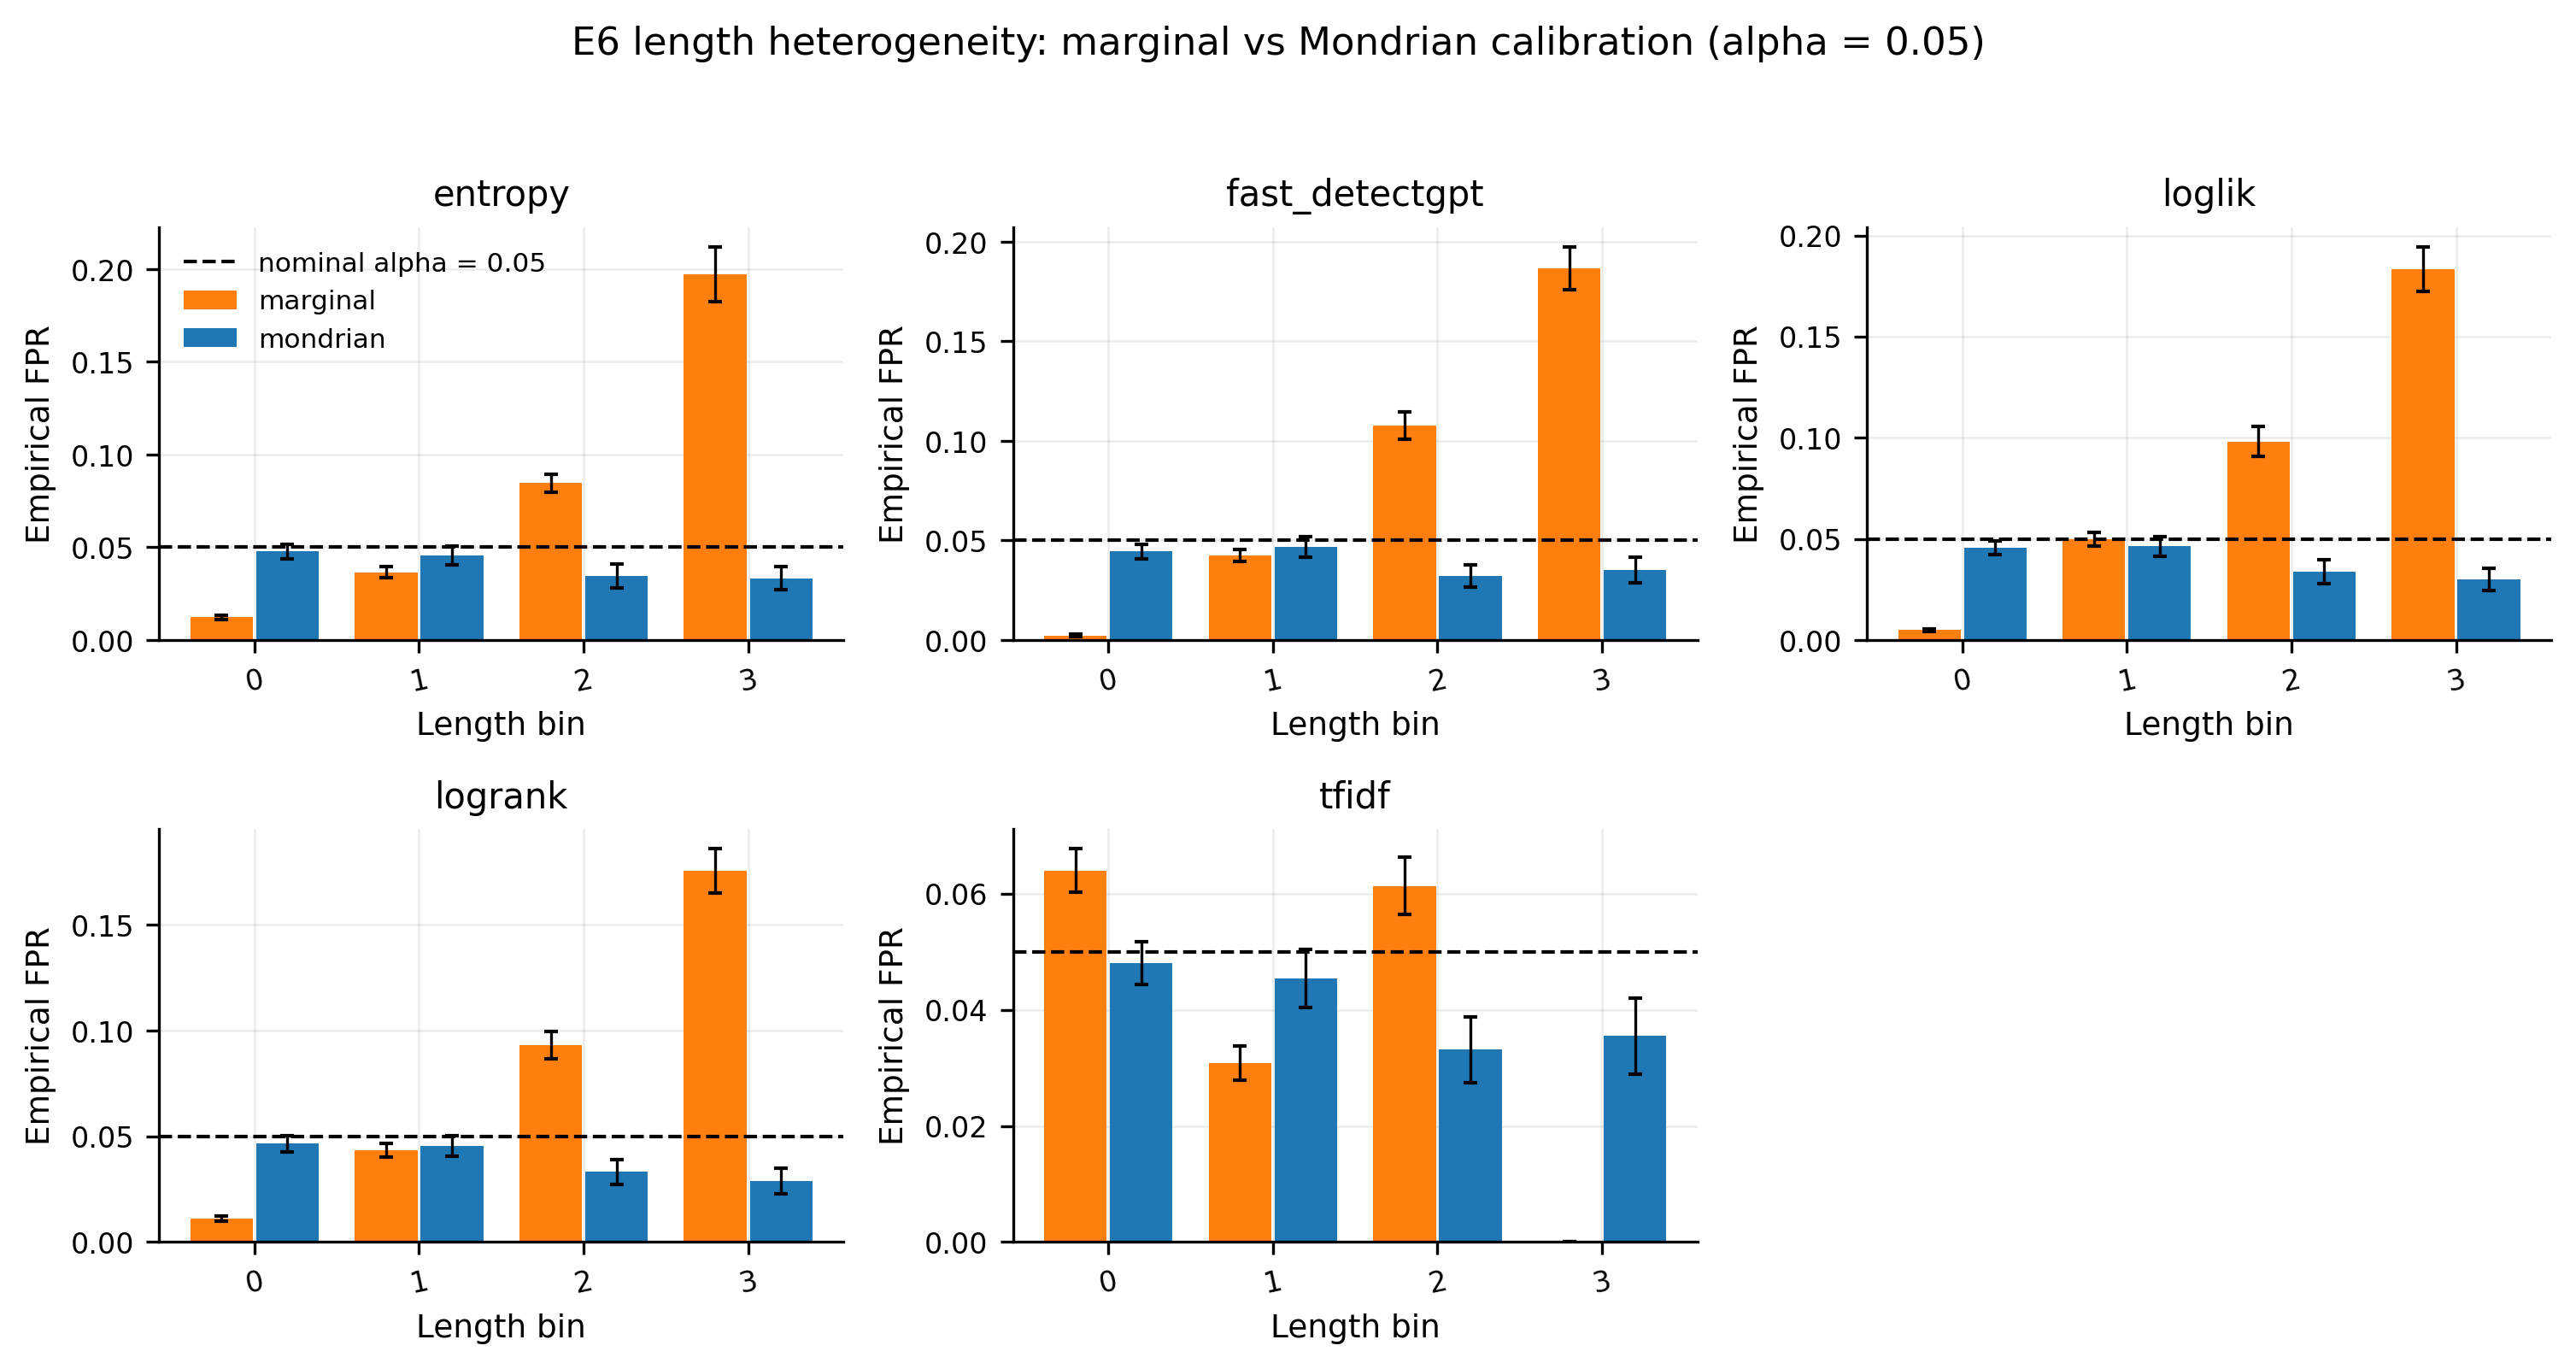
\includegraphics[width=0.9\linewidth]{figures/f5_mondrian.png}
\caption{Marginal vs.\ Mondrian per-length-bin FPR.}
\label{fig:f5_mondrian}
\end{figure}
\subsection{E7: the price of the certificate}
\begin{table}[H]\centering
\caption{Certified power (clean AI text, in-domain).}
\label{tab:e7}
\small
\begin{tabular}{lccc}
\toprule
Score & TPR@$\alpha{=}0.01$ & TPR@$\alpha{=}0.05$ & TPR@$\alpha{=}0.10$ \\
\midrule
Log-likelihood & 0.08 & 0.37 & 0.52 \\
Log-rank & 0.07 & 0.30 & 0.48 \\
Entropy & 0.05 & 0.19 & 0.39 \\
Fast-DetectGPT & 0.03 & 0.24 & 0.39 \\
TF--IDF (supervised) & 0.66 & 0.88 & 0.95 \\
\bottomrule
\end{tabular}
\end{table}
The supervised score detects 88\% of in-domain GPT-4 reviews at a certified 5\% false-accusation rate; zero-shot scores pay heavily for the certificate in-domain but transfer their \emph{power} to unseen generators (Figure~\ref{fig:f7_per_generator}); recall their \emph{validity} caveats above.
\begin{figure}[H]\centering
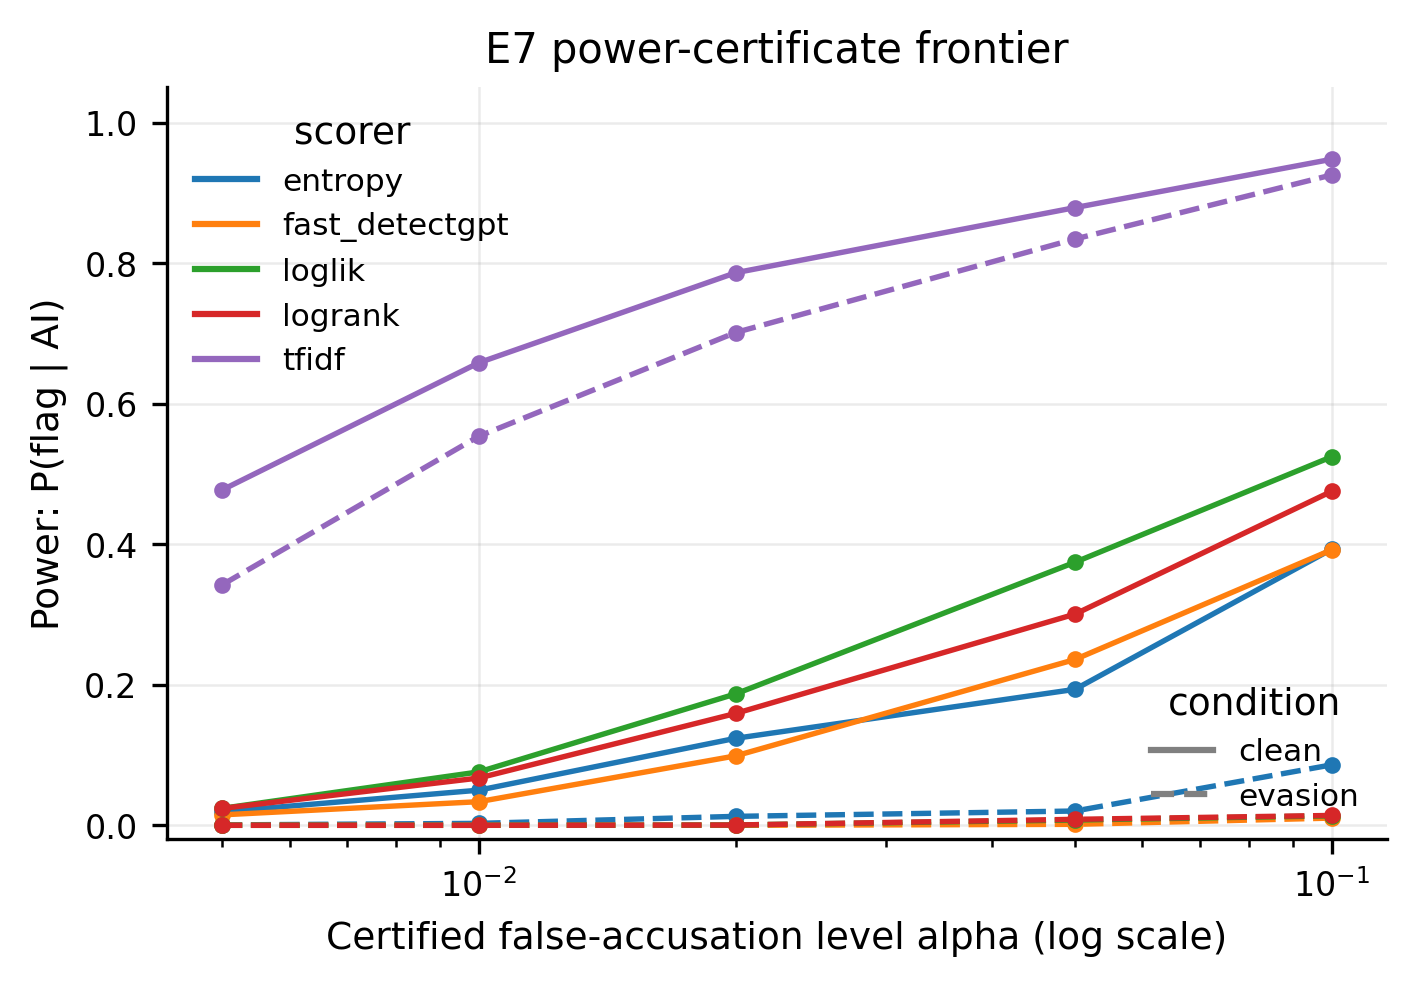
\includegraphics[width=0.9\linewidth]{figures/f6_power_frontier.png}
\caption{Power--certificate frontier per score.}
\label{fig:f6_power_frontier}
\end{figure}
\begin{figure}[H]\centering
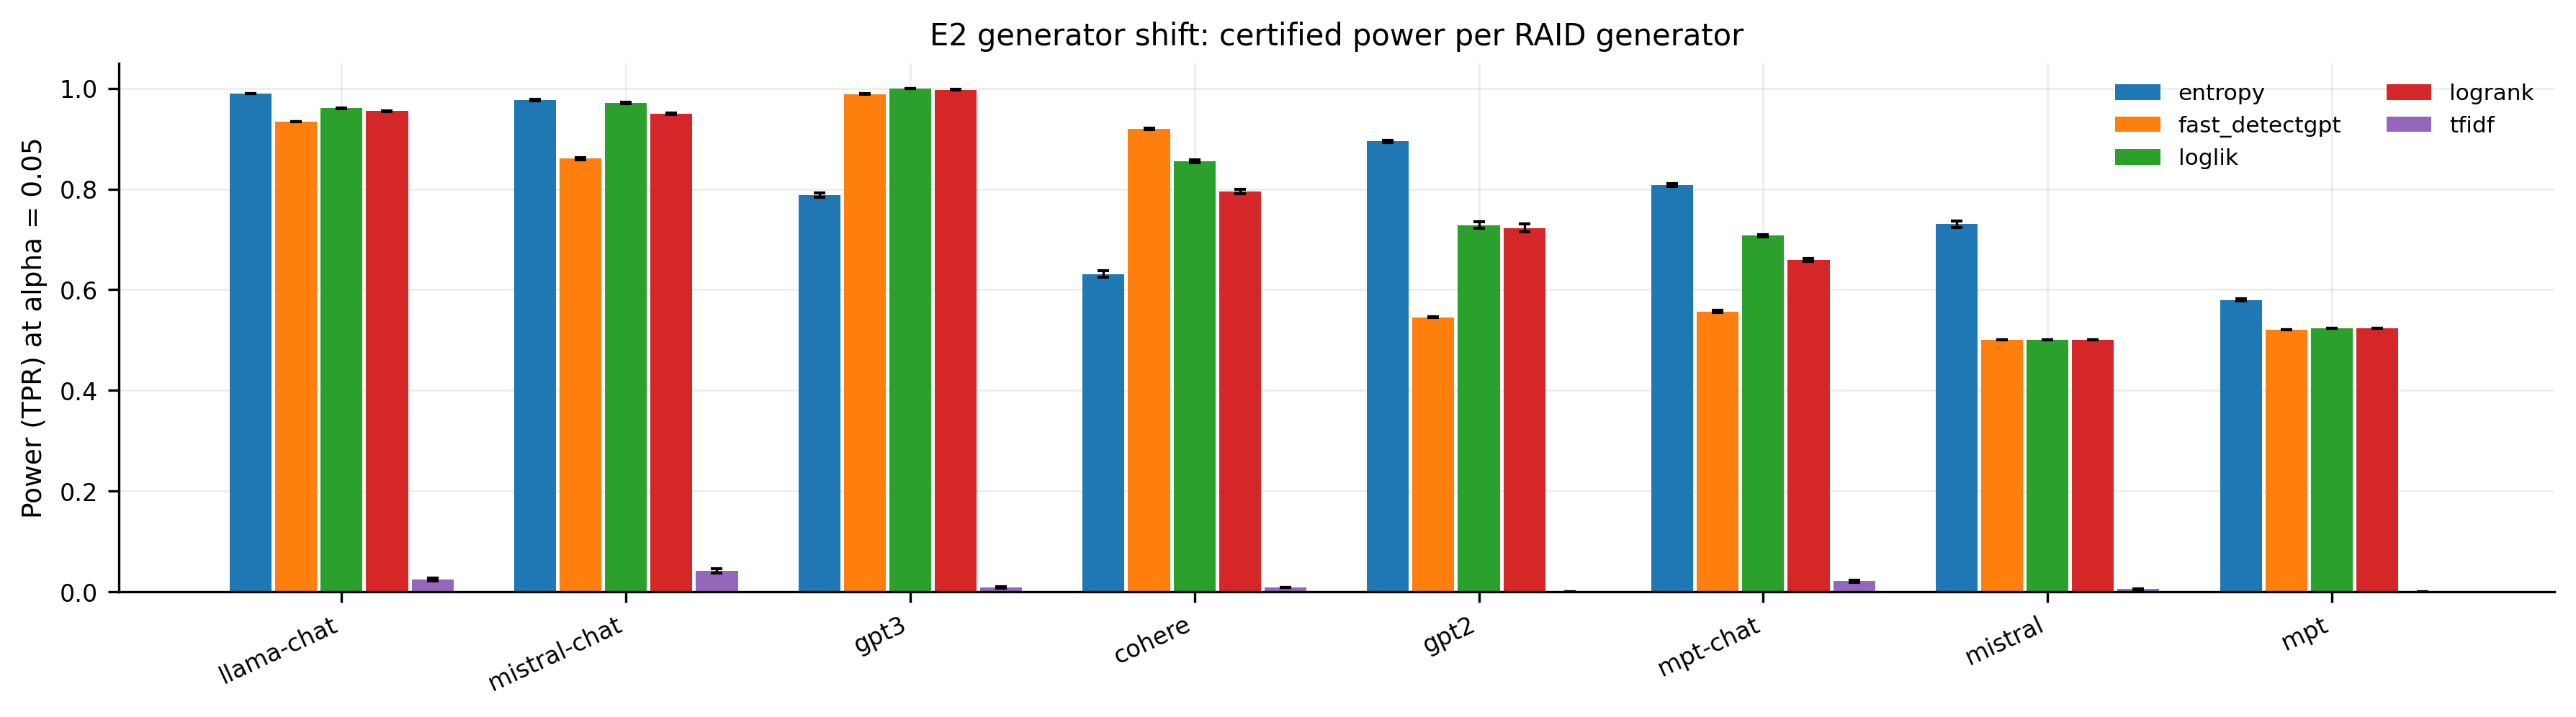
\includegraphics[width=0.95\linewidth]{figures/f7_per_generator.png}
\caption{Certified power per RAID generator.}
\label{fig:f7_per_generator}
\end{figure}
\subsection{E8: editor-aware robust calibration}
\begin{table}[H]\centering
\caption{Editor-aware calibration at $\alpha=0.05$: validity under the modeled editor and the power cost.}
\label{tab:e8}
\small
\begin{tabular}{lcccc}
\toprule
Score & naive FPR (cleaned) & robust FPR (cleaned) & naive TPR & robust TPR \\
\midrule
Log-likelihood & 0.048 & 0.047 & 0.375 & 0.369 \\
Log-rank & 0.047 & 0.046 & 0.303 & 0.297 \\
Entropy & 0.045 & 0.044 & 0.191 & 0.184 \\
Fast-DetectGPT & 0.046 & 0.044 & 0.233 & 0.225 \\
TF--IDF (supervised) & 0.049 & 0.048 & 0.879 & 0.877 \\
\bottomrule
\end{tabular}
\end{table}
With the cleanup editor modeled in calibration, validity holds by construction and the measured power cost is below $0.01$ for every score. In this study the naive certificate already survived cleanup editing, so the robust construction functions as cheap insurance; its value grows with stronger editors, and the guarantee covers any editor whose effect is dominated by the modeled family.
\section{Discussion}
For deployers our results reduce to three rules. First, certify against the humans you will actually judge: the certificate is exact for the calibration population and can be 11$\times$ off for a more fluent one; recalibration per population (or per platform) is cheap and necessary. Second, demand conditional validity: marginal certificates can hide systematic over-accusation of long texts (and, by the population result, of fluent writers); Mondrian calibration over observable strata is a one-line fix. Third, choose the score family by failure mode: supervised content scores buy high certified power in-domain and fail safe under shift; zero-shot likelihood scores transfer power across generators but fail dangerous on shifted humans.
\section{Limitations}\label{sec:limit}
English only; one in-domain corpus (hotel reviews) whose humans skew non-native --- which is what makes the population-shift result vivid, but magnitudes will vary; the cleanup editor under-approximates modern LLM paraphrasers, so E4/E8 bound only the editors tested; GPT-2 is a deliberately modest scorer (the wrapper is scorer-agnostic); and our exact tests certify violations, not their causes --- the fluency mechanism is supported but not isolated. The protocol, released in full, replicates at larger scale directly.
\section{Conclusion}
Distribution-free certificates make AI-text detectors accountable, but only within the human distribution they were calibrated on. We mapped that boundary --- exact in distribution, robust to light editing, broken by population shift, length-biased marginally --- and showed the repairs are cheap. A certificate is a promise about \emph{whom} you calibrated on; deployers should make that promise explicit.
\paragraph{Reproducibility.} All numbers derive from two JSON files produced by \texttt{scripts/run\_all.py} and \texttt{scripts/run\_robust.py}; figures and this paper regenerate from them; conformal correctness is asserted by the test suite.
\begin{thebibliography}{99}\small
\bibitem{vovk} V. Vovk, A. Gammerman, G. Shafer. Algorithmic Learning in a Random World. Springer, 2005.
\bibitem{papadopoulos} H. Papadopoulos, K. Proedrou, V. Vovk, A. Gammerman. Inductive Confidence Machines for Regression. ECML, 2002.
\bibitem{angelopoulos} A. N. Angelopoulos, S. Bates. Conformal Prediction: A Gentle Introduction. Foundations and Trends in Machine Learning, 2023.
\bibitem{mcp} X. Zhang et al. Reliably Bounding False Positives: A Zero-Shot Machine-Generated Text Detection Framework via Multiscaled Conformal Prediction. ACL, 2025.
\bibitem{liang} W. Liang, M. Yuksekgonul, Y. Mao, E. Wu, J. Zou. GPT Detectors Are Biased Against Non-Native English Writers. Patterns, 2023.
\bibitem{raid} L. Dugan et al. RAID: A Shared Benchmark for Robust Evaluation of Machine-Generated Text Detectors. ACL, 2024.
\bibitem{maideup} O. Ignat, X. Xu, R. Mihalcea. MAiDE-up: Multilingual Deception Detection of AI-Generated Hotel Reviews. Findings of NAACL, 2025.
\bibitem{detectgpt} E. Mitchell et al. DetectGPT: Zero-Shot Machine-Generated Text Detection using Probability Curvature. ICML, 2023.
\bibitem{fastdetectgpt} G. Bao et al. Fast-DetectGPT: Efficient Zero-Shot Detection of Machine-Generated Text via Conditional Probability Curvature. ICLR, 2024.
\bibitem{gltr} S. Gehrmann, H. Strobelt, A. M. Rush. GLTR: Statistical Detection and Visualization of Generated Text. ACL Demos, 2019.
\bibitem{solaiman} I. Solaiman et al. Release Strategies and the Social Impacts of Language Models. arXiv:1908.09203, 2019.
\bibitem{krishna} K. Krishna et al. Paraphrasing Evades Detectors of AI-Generated Text, but Retrieval is an Effective Defense. NeurIPS, 2023.
\bibitem{sadasivan} V. S. Sadasivan et al. Can AI-Generated Text be Reliably Detected? arXiv:2303.11156, 2023.
\bibitem{gendler} A. Gendler, T.-W. Weng, L. Daniel, Y. Romano. Adversarially Robust Conformal Prediction. ICLR, 2022.
\bibitem{roberta} Y. Liu et al. RoBERTa: A Robustly Optimized BERT Pretraining Approach. arXiv:1907.11692, 2019.
\end{thebibliography}
\end{document}
